% This must be in the first 5 lines to tell arXiv to use pdfLaTeX, which is strongly recommended.
\pdfoutput=1
% In particular, the hyperref package requires pdfLaTeX in order to break URLs across lines.

\documentclass[11pt]{article}
\usepackage{graphicx}
\usepackage{subcaption}
\usepackage{float}

% Remove the "review" option to generate the final version.
\usepackage[]{ACL2023}

% Standard package includes
\usepackage{times}
\usepackage{latexsym}
\usepackage{graphicx}
% For proper rendering and hyphenation of words containing Latin characters (including in bib files)
\usepackage[T1]{fontenc}
% For Vietnamese characters
% \usepackage[T5]{fontenc}

% This assumes your files are encoded as UTF8
\usepackage[utf8]{inputenc}

% This is not strictly necessary, and may be commented out.
% However, it will improve the layout of the manuscript,
% and will typically save some space.
\usepackage{microtype}

% This is also not strictly necessary, and may be commented out.
% However, it will improve the aesthetics of text in
% the typewriter font.
\usepackage{inconsolata}

\usepackage{multirow}
\usepackage{graphicx}
\usepackage{fancyhdr}
% If the title and author information does not fit in the area allocated, uncomment the following
%
%\setlength\titlebox{<dim>}
%
% and set <dim> to something 5cm or larger.

\title{Federated Hate-Speech Recognition}
% Author information can be set in various styles:
% For several authors from the same institution:
% \author{Author 1 \and ... \and Author n \\
%         Address line \\ ... \\ Address line}
% if the names do not fit well on one line use
%         Author 1 \\ {\bf Author 2} \\ ... \\ {\bf Author n} \\
% For authors from different institutions:
% \author{Author 1 \\ Address line \\  ... \\ Address line
%         \And  ... \And
%         Author n \\ Address line \\ ... \\ Address line}
% To start a seperate ``row'' of authors use \AND, as in
% \author{Author 1 \\ Address line \\  ... \\ Address line
%         \AND
%         Author 2 \\ Address line \\ ... \\ Address line \And
%         Author 3 \\ Address line \\ ... \\ Address line}

\author{
    Ashkan Vedadi Gargary \\ University of California, Riverside\\ \texttt{aveda002@ucr.edu} 
    \AND
    Aditya Mohan Gupta \\ University of California, Riverside\\ \texttt{agupt166@ucr.edu}
  }

\begin{document}
\maketitle
\pagestyle{fancy}
\fancyhf{}
\fancyfoot[C]{\thepage}
\renewcommand{\headrulewidth}{0pt}
\pagenumbering{arabic}
\begin{abstract}
\textit{Content warning: This paper contains unfiltered content reported by Hate Speech Datasets that may be offensive to readers.}

Hate speech recognition is critical for maintaining healthy online communities. This paper explores the efficacy of federated learning (FL) in enhancing hate speech detection models compared to traditional centralized approaches. We evaluate several state-of-the-art centralized models, including BERT-based models, Random Forests, Decision Trees, K-nearest neighbors (KNN), and Logistic Regression. Additionally, we introduce two federated methods based on Neural Networks and TinyBERT, facilitating distributed training across multiple devices while preserving data privacy.

Our experimental results, benchmarked using F1 score and accuracy metrics, indicate that FL models outperform classical centralized models by a significant margin, achieving over $6\%$ higher accuracy. Moreover, our FL models perform almost as well as the centralized TinyBERT-based model. These findings underscore the potential of Federated Learning to improve the robustness and performance of hate speech recognition systems, paving the way for more secure and effective content moderation strategies.


\end{abstract}

\section{Introduction}
Hate speech recognition is important in natural language processing (NLP) and machine learning (ML), driven by the need to foster safer online environments. The rise of social media has increased the volume of harmful content, challenging community standards and public safety. Effective hate speech detection systems are essential for mitigating harmful rhetoric, protecting vulnerable groups, and maintaining the integrity of online discourse.

Traditional centralized machine learning approaches have been widely used for hate speech detection, including BERT-based models, random forests, decision trees, K-Nearest Neighbors (KNN), and logistic regression. These models are typically trained on large datasets aggregated in a single location, raising concerns over data privacy and security. 

In recent years, Federated Learning has become popular, with more people wanting machine learning models that work on many devices without sharing local files. This method allows clients to train models on their data and only share models update, not the actual data, with a central server. This keeps data private and facilitates the learning process.


Federated Learning is particularly beneficial for hate speech recognition. FL harnesses multiple devices' computational power and data diversity without compromising privacy. This decentralized approach reduces risks associated with centralized data collection and enhances the model's generalization ability across varied contexts. 

\paragraph{Problem Definition} 
We propose an FL-based model for Hate Speech recognition and show that it can outperform centralized models by achieving over $6\%$ higher accuracy. We also try to compare different methods of Federated-based recognition with TinyBert Classifier. We mainly focus on the datasets that classify a prompt or message into two groups: (i) Hate-Full and (ii) Non-Hate-Full.

\paragraph{Beginning Objectives}
Our main objectives can be summarized into these groups:
\begin{itemize}
    \item \textbf{Finding Related Datasets:} 
    Hate speech encompasses various sub-problems, such as Racism, Sexism, and Cyberbullying. This work focuses primarily on general hate speech recognition, where content is classified as hateful or not, without focusing on specific subcategories. Our objectives include identifying related datasets and adapting them to our needs, ensuring we have sufficient data from different sources for fair evaluation in the FL setup.
    
    \item \textbf{Data Pre-Processing:} 
    Addressing class imbalance is crucial in hate speech detection. Data pre-processing is one of our main goals to ensure the data is suitable for our models. Additionally, for centralized models, we need to merge datasets from different sources.
    
    \item \textbf{Re-implementing State-of-the-Art Centralized Methods:} Many centralized models, such as Random Forest, KNN, Decision Trees, and Logistic Regression, have shown high accuracy in hate speech recognition. Recent research also utilizes BERT classifiers. Our objective is to re-implement these models to facilitate fair comparisons.
    
    \item \textbf{Federating Best Centralized Models:} To develop federated models, our first step is to adapt best current centralized models to a federated learning framework.
    
    \item \textbf{Reproducing Current Federated Models:} Another objective is to reproduce existing state-of-the-art federated hate speech recognition models.

    \item \textbf{Comparing All Models:} Ultimately, we aim to compare all models and discuss their performance fairly.
\end{itemize}









\section{Related Work}

Significant research and development have been conducted in the fields of centralized and federated learning, reflecting the evolving priorities in machine learning, particularly regarding data privacy and computational efficiency.

In centralized learning, data is aggregated into a single repository for model training. This traditional approach has facilitated breakthroughs in various domains. For instance, the development of convolutional neural networks (CNNs) by LeCun et al. (1989) revolutionized image recognition tasks, and subsequent improvements by Krizhevsky et al. (2012) with AlexNet demonstrated the power of deep learning on large-scale datasets. Additionally, centralized learning has proven effective in natural language processing with the introduction of the Transformer model by Vaswani et al. (2017), which underpins many modern NLP applications.

Conversely, federated learning (FL) emerged to address privacy and data distribution concerns inherent in centralized learning. Introduced by McMahan et al. (2017), FL enables model training across multiple decentralized devices, sharing only model updates rather than raw data. This approach is crucial in sensitive domains like healthcare, where Sheller et al. (2020) demonstrated the viability of FL in medical imaging, and in mobile applications, as explored by Hard et al. (2018) with Google's Gboard. Recent research has focused on optimizing communication efficiency (Konecny et al., 2016) and improving model aggregation methods (Bonawitz et al., 2019), addressing the unique challenges posed by non-IID data distributions (Zhao et al., 2018).


\section{Background}

Centralized learning, the traditional method of training machine learning models, involves collecting data from multiple sources into a single location. This centralized approach has the advantage of creating comprehensive datasets, enhancing model accuracy and robustness. However, it raises significant concerns about data privacy, security, and scalability. The requirement to transfer large amounts of data to a central server can lead to privacy breaches and increased vulnerability to cyberattacks.

On the other hand, Federated learning is a decentralized approach designed to mitigate these issues. By keeping data on local devices and only sharing model updates, FL preserves data privacy and reduces the risk of breaches. This method is particularly beneficial in contexts where data is sensitive or subject to strict privacy regulations, such as in healthcare or finance. FL also leverages the computational power of edge devices, potentially reducing the central server's load and enhancing scalability. However, FL introduces new challenges, such as ensuring efficient communication between devices, handling heterogeneous data, and achieving robust model aggregation.

The evolution from centralized to federated learning reflects a broader shift towards prioritizing data privacy and distributed computing power. Both approaches have their merits and are suited to different scenarios, complementing the broader landscape of machine learning research and application.

\section{Data}
\label{sec:dataset}
We combine our dataset using the mentioned dataset proposed by ~\cite{FORTUNA2021102524}. 

\subsection{Selected Dataset} We reuse 3 of the 9 datasets used by ~\cite{FORTUNA2021102524} to form our combine datasets. We perform a stratified split of all training data into training ($70\%$) and testing ($30\%$) sets.
\subsubsection{Kaggle (1): Twitter Hate Speech ~\cite{agarwal2024twitter}}
One of the datasets from Twitter combines many different Twitter datasets by having 49159 rows. Their dataset only contains tweets and labels.

\subsubsection{Kaggle (2): Cyberbullying ~\cite{elsafoury2020cyberbullying}}
One of the largest datasets from Wikipedia contains 159571 rows. Their datasets contain many different things and provide different datasets for different classification problems. However, we only use \textit{toxicity\_parsed\_dataset.csv}, which is used for the hate-speech classifier.

\subsubsection{Davidson ~\cite{davidson2017automated}} 
\label{sec:davidson}
It is one of the most well-used datasets among all of the existing datasets, including tweets from Twitter. Davidson dataset contains 24783 rows that contain three labels: (i) hate full, (ii) offensive language, and (iii) neither. Since our model's focus is only on hate speech recognition, we remove offensive language texts and only keep the hateful and non-hateful rows. After refactoring the datasets, it has 5593 rows. 

\subsection{Data Cleaning} We have two aspects of data cleaning. First, as mentioned in Section \ref{sec:davidson}, we removed offensive language and focused only on hateful and non-hateful. Second, we cleaned each text by converting it to lowercase and removing unnecessary characters (e.g. @, Non-Alphanumeric, URLs). 

\begin{figure}[t]
    \centering
    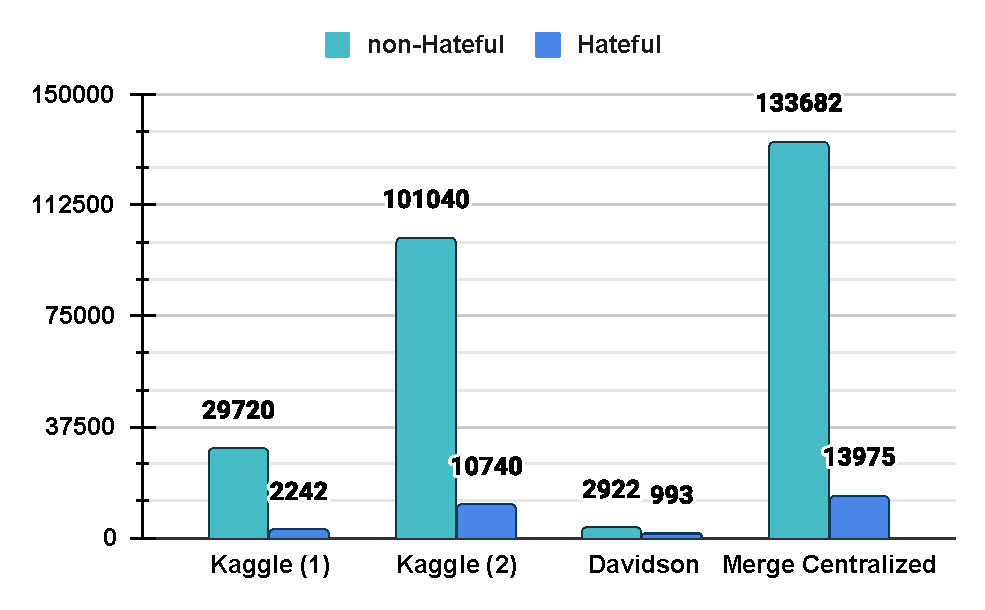
\includegraphics[width=.5\textwidth]{images/data-imbalance.pdf}
    \caption{Data Imbalance Among Different Train Set of Each Dataset.}
    \label{fig:data-imbalance}
\end{figure}

\subsection{Up-sampling} 
As mentioned in Figure \ref{fig:data-imbalance}, we have a huge class imbalance by checking the count of each label in each dataset. 
We address issues of extreme class imbalance by augmenting the hateful words and generating new texts on train sets based on them to balance the size of hateful and non-hateful texts. In Appendix \ref{sec:data-visualization}, we present data visualization of different classes before and after data augmentation.


\section{Centralized Methods}

\subsection{Decision Trees}
The Decision Tree classifier uses a tree-like model of decisions based on the \textit{entropy} criterion to split nodes, optimizing the classification process by maximizing information gain~\cite{song2015decision}. We used the \texttt{DecisionTreeClassifier} from the scikit-learn library for our decision tree implementation. To ensure reproducibility, the model was configured with the criterion set to \textit{entropy} and a random state of $0$. This setup allows the model to make splits based on the information gain, optimizing the decision-making process at each node.

\subsection{Random Forrest}
The Random Forest classifier employs an ensemble of many decision trees, using \textit{entropy} as the criterion for splits, to enhance prediction accuracy and robustness through aggregation~\cite{rigatti2017random}. We implemented a Random Forest classifier using scikit-learn's \texttt{RandomForestClassifier}. The model was initialized with $10$ estimators, using \textit{entropy} as the criterion for information gain calculation and a random state of $0$. This ensemble method uses multiple decision trees to improve the robustness and accuracy of the predictions.

\subsection{KNNs}
The K-Nearest Neighbors classifier classifies data points based on the majority class among the nearest neighbors, utilizing the Minkowski distance metric with a Euclidean distance configuration~\cite{peterson2009k}.
We utilized scikit-learn's \texttt{KNeighborsClassifier} for the K-Nearest Neighbors classifier. The model was set with $5$ neighbors and employed the Minkowski distance metric with a power parameter (p) of $2$, equivalent to the Euclidean distance. This method classifies a sample based on the majority class among its nearest neighbors.


\subsection{Logistic Regression}
Logistic Regression is a linear model used for binary classification, which predicts the probability of a class membership based on input features, serving as a baseline comparison in this study~\cite{lavalley2008logistic}.
The Logistic Regression model was implemented using scikit-learn's \texttt{LogisticRegression}, with a random state of $0$ to ensure consistent results across runs. This linear model is well-suited for binary classification tasks and was used as a baseline for comparison.

\subsection{Tiny-Bert}
For our BERT-based model, we employed Tiny-BERT, a compact version of the BERT model~\cite{bhargava2021generalization, DBLP:journals/corr/abs-1908-08962}. Tiny-Bert has a total of $4$ million parameters and $2$ hidden layers with $128$ hidden dimension. Tiny-Bert is $7x$ smaller and $9x$ faster than BERT while achieving $96\%$ of its performance~\cite{jiao2020tinybert}. We used the \texttt{BertTokenizer} and \texttt{BertForSequenceClassification} from the Hugging Face library, pretrained on the \textit{prajjwal1/bert-tiny} model with $2$ output labels for binary classification. The model was trained using the Trainer API from Hugging Face's Transformers library, with a training configuration that included $5$ epochs, a batch size of $16$, $10$ warmup steps, $0.01$ as weight decay, and logging every $10$ steps. The training was performed on a GPU.






\section{Federated Methods}

We propose two main methods for federated implementation. First, classic tokenization and neural network design are used for binary classification with FedProx as aggregated method. Second, we federated our Centralized TinyBert Classifier using PySyft with FedAVG as aggregate method for our training process.


\subsection{Federated Learning Setup}

Federated learning is employed to train the model across multiple clients without transferring the data to a central server. This approach ensures data privacy and security while leveraging distributed computational resources. Both implementations utilize the same setup, involving the following steps:


\begin{itemize}
    \item \textbf{Client Initialization:} We initialize multiple virtual clients to simulate a federated learning environment. Each client represents a separate entity holding a portion of the training data. 
    \item \textbf{Data Distribution:} The training dataset is partitioned and distributed among the clients. Each client receives a unique subset of the data to perform local training.
    \item \textbf{Model Training:} The model is trained locally on each client's data. The local models are updated based on the data subsets they hold.
    \item \textbf{Model Aggregation:} After local training, the updated model parameters are sent to a central server for aggregation. The server averages the parameters to create a global model. The Federated Averaging (FedAvg) algorithm is used to combine the model updates from all clients. 
    \item \textbf{Iterative Process:} The training and aggregation steps are repeated iteratively over multiple epochs until the model converges or achieves satisfactory performance. We set the number of iterations to $10$.
\end{itemize}

This federated learning setup ensures that the model can learn from a diverse dataset while preserving the privacy of each client's data. By keeping the data local and only sharing model updates, we mitigate the risks associated with data breaches and ensure compliance with privacy regulations.

\subsection{Federated Neural Networks with FedProx}

The FedProx algorithm is implemented to add a proximal term to the loss function. This term penalizes deviations from the global model parameters, thus stabilizing training in heterogeneous environments.

\subsubsection{FedProx}

The implemented model for hate speech detection is a simple neural network designed for binary classification. The architecture consists of:

\begin{itemize}
    \item \textbf{Input Layer:} This layer accepts feature vectors derived from the preprocessed text data.
    \item \textbf{Hidden Layers:} One or more hidden layers with ReLU (Rectified Linear Unit) activation functions to introduce non-linearity and enable the model to learn complex patterns in the data.
    \item \textbf{Output Layer:} A single neuron with a sigmoid activation function to output the probability of the text being classified as hate speech. The sigmoid function is suitable for binary classification as it maps the output to a value between 0 and 1.
\end{itemize}

The choice of a simple neural network architecture is motivated by the need for efficient training and inference in a federated learning setting, where computational resources on client devices might be limited. The architecture is flexible enough to be extended with additional layers or neurons if required to handle more complex data or achieve higher performance.




\subsection{Federated TinyBert with FedAVG}
We utilize our best centralized model, TinyBERT, for our federated setup. By using virtual machines in the PySyft library, we simulate the federated environment. For our BERT-based model, we employed Tiny-BERT, a compact version of the BERT model~\cite{bhargava2021generalization, DBLP:journals/corr/abs-1908-08962}. As mentioned earlier, Tiny-Bert has a total of $4$ million parameters and $2$ hidden layers with $128$ hidden dimension. Tiny-Bert is $7x$ smaller and $9x$ faster than BERT while achieving $96\%$ of its performance~\cite{jiao2020tinybert}. We used the \texttt{BertTokenizer} and \texttt{BertForSequenceClassification} from the Hugging Face library, pretrained on the \textit{prajjwal1/bert-tiny} model with $2$ output labels for binary classification. The model was trained using the Trainer API from Hugging Face's Transformers library, with a training configuration that included $5$ epochs, a batch size of $16$, $10$ warmup steps, $0.01$ as weight decay, and logging every $10$ steps. The training was performed on a GPU.


\section{Experiments and Results}
This section presents and compares our proposed Federated and Centralized evaluation results with each other. All the source code and datasets are available online for results reproduction, mentioned in Section \ref{sec:materials}.

\subsection{Experiment Setup}
In this section, we summarize the Hardware and Libraries that we utilized. We also review the datasets and comparison methodologies for both centralized and federated setups. 

\subsubsection{Hardware and Software}
We utilized the free version of the Google Colab research system for our experimental results. We employed scikit-learn libraries to implement the centralized models, Hugging Face to fine-tune the necessary models, and the Syft library to incorporate federated learning into our code.


\subsubsection{Dataset}
As mentioned in Section \ref{sec:dataset}, we have three different datasets: (i) Kaggle (1), (ii) Kaggle (2), and (iii) Davidson. By pre-processing and up-sampling the data, we have three training sets for both centralized and federated methods. We also create one additional dataset, which results from merging these three datasets, and call it (iv) the Merged dataset. More information on the dataset is summarized in Table \ref{tab:dataset}.


\begin{table}[]
\centering
\caption{Data Information}
\label{tab:dataset}
\resizebox{\columnwidth}{!}{%
\begin{tabular}{|l|rrr|r|}
\hline
\textbf{}           & \multicolumn{3}{l|}{\textbf{Train}}                               & \multicolumn{1}{l|}{\textbf{Test}} \\ \hline
\textbf{Data} &
  \multicolumn{1}{l|}{\textbf{\#Size}} &
  \multicolumn{1}{l|}{\textbf{\#non-Hateful}} &
  \multicolumn{1}{l|}{\textbf{\#Hateful}} &
  \multicolumn{1}{l|}{\textbf{\#Size}} \\ \hline
\textbf{Kaggle (1)} & \multicolumn{1}{r|}{31962}  & \multicolumn{1}{r|}{29720}  & 2242  & 17197                              \\ \hline
\textbf{Kaggle (2)} & \multicolumn{1}{r|}{111780} & \multicolumn{1}{r|}{101040} & 10740 & 47905                              \\ \hline
\textbf{Davidson}   & \multicolumn{1}{r|}{3915}   & \multicolumn{1}{r|}{2922}   & 993   & 1678                               \\ \hline
\textbf{Merged}     & \multicolumn{1}{r|}{147657} & \multicolumn{1}{r|}{133682} & 13975 & 66780                              \\ \hline
\end{tabular}%
}
\end{table}

\subsubsection{Approaches}
For centralized approaches, we compare Decision Tree (DT), Logistic Regression (LR), K-nearest neighbors (KNN), Random Forest (RF), and TinyBert (TB) classifier. According to our resources, the TinyBert classifier is the best available mechanism. Then, we use the Bert classifier (TB) and compare it with our Federated Neural Network and Federated TinyBert model. 

\subsection{Centralized Methods}
In this section, we focus on centralized methods to find the best-centralized methods. First, we compare the performance of different clients.
\subsubsection{Each Dataset}
As shown in Table \ref{tab:centralized-seperated}, all models perform strongly on the validation set. This is mainly due to the upsampling applied during implementation, which, while beneficial for training, tends to increase the risk of overfitting. Therefore, we also report test accuracy and F1 scores for a more balanced evaluation.

Random Forest (RF) achieves the best performance among classical machine learning models. However, the performance gap is substantial compared to the TinyBERT classifier, which outperforms all other classical machine learning models by a significant margin.

TinyBERT achieves over $91\%$ accuracy across all three datasets. One notable exception is the Davidson dataset, which shows lower performance. This is because, after removing one of its classes to fit our binary classification problem (0 for non-hateful and 1 for hateful), the dataset is left with fewer instances, affecting the model's performance.

% Please add the following required packages to your document preamble:
% \usepackage{multirow}
% \usepackage{graphicx}
\begin{table}[]
\centering
\caption{Compare the Train and Accuracy of each dataset. }
\label{tab:centralized-seperated}
\resizebox{\columnwidth}{!}{%
\begin{tabular}{|c|c|cc|cc|}
\hline
\multicolumn{1}{|l|}{\multirow{2}{*}{\textbf{Datasets}}} &
  \multirow{2}{*}{\textbf{Model}} &
  \multicolumn{2}{c|}{\textbf{Validation (20\%)}} &
  \multicolumn{2}{c|}{\textbf{Test (30\%)}} \\ \cline{3-6} 
\multicolumn{1}{|l|}{} &
   &
  \multicolumn{1}{c|}{\textbf{Accuracy}} &
  \textbf{F1} &
  \multicolumn{1}{c|}{\textbf{Accuracy}} &
  \textbf{F1} \\ \hline
\multirow{5}{*}{\textbf{Kaggle (1)}} & DT          & \multicolumn{1}{c|}{97.49\%}          & 97.40\%          & \multicolumn{1}{c|}{67.24\%}          & 79.89\%          \\ \cline{2-6} 
                                     & LR          & \multicolumn{1}{c|}{94.03\%}          & 93.90\%          & \multicolumn{1}{c|}{51.86\%}          & 66.62\%          \\ \cline{2-6} 
                                     & KNN         & \multicolumn{1}{c|}{96.57\%}          & 96.43\%          & \multicolumn{1}{c|}{67.24\%}          & 79.89\%          \\ \cline{2-6} 
                                     & RF          & \multicolumn{1}{c|}{98.67\%}          & 98.64\%          & \multicolumn{1}{c|}{71.03\%}          & 82.75\%          \\ \cline{2-6} 
                                     & \textbf{TB} & \multicolumn{1}{c|}{\textbf{98.36\%}} & \textbf{98.36\%} & \multicolumn{1}{c|}{\textbf{95.33\%}} & \textbf{95.47\%} \\ \hline
\multirow{5}{*}{\textbf{Kaggle (2)}} & DT          & \multicolumn{1}{c|}{46.70\%}          & 52.61\%          & \multicolumn{1}{c|}{51.82\%}          & 66.60\%          \\ \cline{2-6} 
                                     & LR          & \multicolumn{1}{c|}{90.83\%}          & 91.01\%          & \multicolumn{1}{c|}{78.67\%}          & 87.91\%          \\ \cline{2-6} 
                                     & KNN         & \multicolumn{1}{c|}{90.09\%}          & 89.18\%          & \multicolumn{1}{c|}{87.33\%}          & 93.22\%          \\ \cline{2-6} 
                                     & RF          & \multicolumn{1}{c|}{98.44\%}          & 98.42\%          & \multicolumn{1}{c|}{58.85\%}          & 73.06\%          \\ \cline{2-6} 
                                     & \textbf{TB} & \multicolumn{1}{c|}{\textbf{97.73\%}} & \textbf{97.72\%} & \multicolumn{1}{c|}{\textbf{94.00\%}} & \textbf{94.43\%} \\ \hline
\multirow{5}{*}{\textbf{Davidson}}   & DT          & \multicolumn{1}{c|}{95.95\%}          & 95.80\%          & \multicolumn{1}{c|}{54.35\%}          & 67.90\%          \\ \cline{2-6} 
                                     & LR          & \multicolumn{1}{c|}{96.12\%}          & 96.00\%          & \multicolumn{1}{c|}{55.42\%}          & 68.52\%          \\ \cline{2-6} 
                                     & KNN         & \multicolumn{1}{c|}{85.29\%}          & 86.05\%          & \multicolumn{1}{c|}{54.35\%}          & 67.90\%          \\ \cline{2-6} 
                                     & RF          & \multicolumn{1}{c|}{96.01\%}          & 95.86\%          & \multicolumn{1}{c|}{54.89\%}          & 68.34\%          \\ \cline{2-6} 
                                     & \textbf{TB} & \multicolumn{1}{c|}{\textbf{92.13\%}} & \textbf{92.13\%} & \multicolumn{1}{c|}{\textbf{91.90\%}} & \textbf{91.96\%} \\ \hline
\multirow{5}{*}{\textbf{Merge}}      & DT          & \multicolumn{1}{c|}{96.36\%}          & 96.24\%          & \multicolumn{1}{c|}{60.78\%}          & 74.59\%          \\ \cline{2-6} 
                                     & LR          & \multicolumn{1}{c|}{94.96\%}          & 97.26\%          & \multicolumn{1}{c|}{85.35\%}          & 88.04\%          \\ \cline{2-6} 
                                     & KNN         & \multicolumn{1}{c|}{91.46\%}          & 95.37\%          & \multicolumn{1}{c|}{60.78\%}          & 74.59\%          \\ \cline{2-6} 
                                     & RF          & \multicolumn{1}{c|}{98.12\%}          & 98.09\%          & \multicolumn{1}{c|}{73.87\%}          & 84.61\%          \\ \cline{2-6} 
                                     & TB          & \multicolumn{1}{c|}{\textbf{97.20\%}} & \textbf{97.20\%} & \multicolumn{1}{c|}{\textbf{93.31\%}} & \textbf{93.96\%} \\ \hline
\end{tabular}%
}
\end{table}


\subsubsection{Merged Datasets}
To compare our models using merged datasets, we combined all three datasets into a single dataset and reran all the experiments. We achieved an accuracy and F1 score of $93\%$. Notably, the validation and test accuracy and F1 scores are almost identical, indicating no signs of overfitting in the results.

One interesting result is the increase in the Accuracy and F1 score in classical ML due to merging the datasets.

We will further compare the federated methods with the Centralized TinyBERT classifier.




\subsection{Federated Methods}
In this section, we first compare various federated methods. Subsequently, we contrast the performance of the best federated setup with the TinyBERT classifier on merged datasets, representing the best-centralized method.



\subsubsection{Federated Hate-Speech Recognition Comparison}

We applied the Federated Neural Networks model with FedProx aggregation to binary hate speech detection datasets. The model was trained over several iterations (ranging from 1 to 10), with accuracy recorded after each iteration. The training process demonstrated that the FedProx algorithm effectively maintained high accuracy while preserving data privacy across multiple clients. The final accuracy achieved was satisfactory, confirming the efficacy of this approach.

To visualize the training progress, Figure \ref{fig:results-1} shows the accuracy and loss over different iterations. The graph illustrates the improvement in model accuracy with each epoch, highlighting the stability and effectiveness of the FedProx algorithm in a federated setting.

In contrast, we applied Federated TinyBERT with FedAVG aggregation to the hate speech detection datasets over 10 iterations. Due to GPU resource limitations, we avoided upsampling. Figure \ref{fig:results-2} demonstrates the increase in accuracy over 10 iterations.

Both models achieved $92\%$ accuracy on the test sets after $10$ iterations.

\subsubsection{Centralized Vs. Federated}
As shown in Table \ref{tab:all-results}, our implementation of both federated methods outperforms traditional centralized methods. Additionally, when compared to the centralized TinyBERT, our federated approaches achieve nearly the same accuracy after 10 iterations, while providing enhanced privacy.
\begin{table}[]
\centering
\small
\caption{Centralized and Federated Models Comparison}
\label{tab:all-results}
\begin{tabular}{|c|c|c|}
\hline
\textbf{\begin{tabular}[c]{@{}c@{}}Training\\ Model\end{tabular}} &
  \textbf{\begin{tabular}[c]{@{}c@{}}Aggregation\\ Method\end{tabular}} &
  \textbf{\begin{tabular}[c]{@{}c@{}}Test\\ Accuracy\end{tabular}} \\ \hline
\textbf{Centralized DT}           & N/A     & 60.78\% \\ \hline
\textbf{Centralized RF}           & N/A     & 73.87\% \\ \hline
\textbf{Centralized LR}           & N/A     & 85.35\% \\ \hline
\textbf{Centralized KNN}          & N/A     & 60.78\% \\ \hline
\textbf{Centralized TinyBert}     & N/A     & 93.31\% \\ \hline
\textbf{Federated Neural Network} & FedProx & 90.35\% \\ \hline
\textbf{Federated TinyBert}       & FedAVG  & 90.80\% \\ \hline
\end{tabular}
\end{table}

% \subsubsection{Graphs}

% To visualize the training progress, the accuracy over epochs was plotted. The graph below shows the model's accuracy improvement with each epoch, highlighting the stability and effectiveness of the FedProx algorithm in a federated setting.
% \begin{figure*}[H]
%     \centering
%     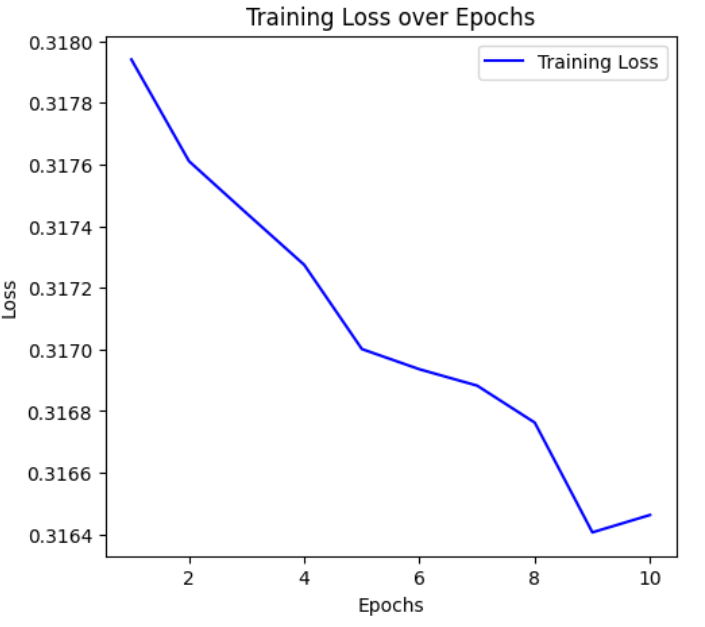
\includegraphics[width=0.45\linewidth]{images/results1.PNG}
%     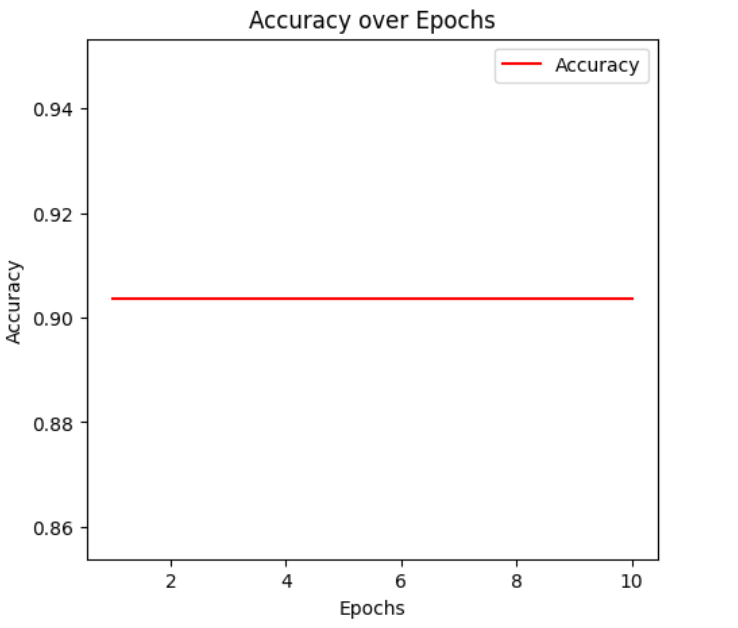
\includegraphics[width=0.45\linewidth]{images/Results2.PNG}
%     \caption{Training Loss (left) and Accuracy (right) over Epochs}
%     \label{fig:loss-1}
% \end{figure*}

\begin{figure*}[h]
    \centering
    \begin{subfigure}[b]{0.43\textwidth}
        \centering
        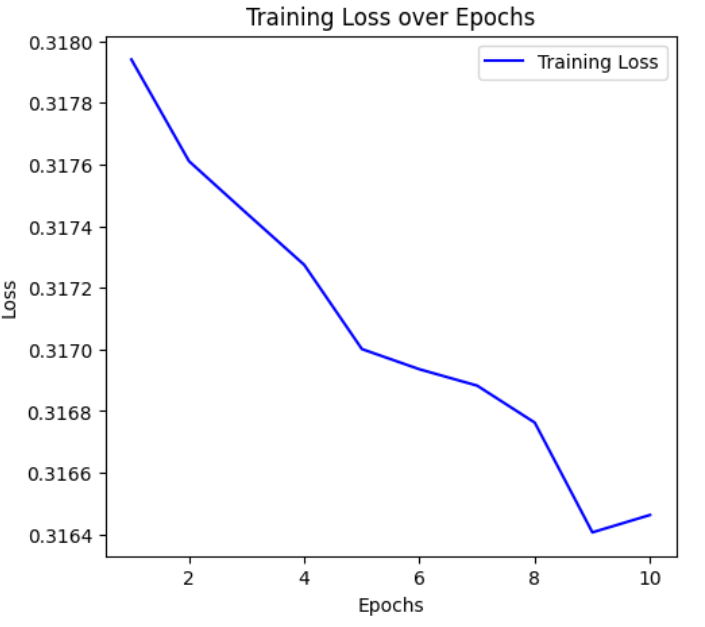
\includegraphics[width=\textwidth]{images/results1.PNG}
        \caption{Training Loss over 10 iterations}
        \label{fig:los-2} % Corrected label
    \end{subfigure}
    \hfill
    \begin{subfigure}[b]{0.45\textwidth}
        \centering
        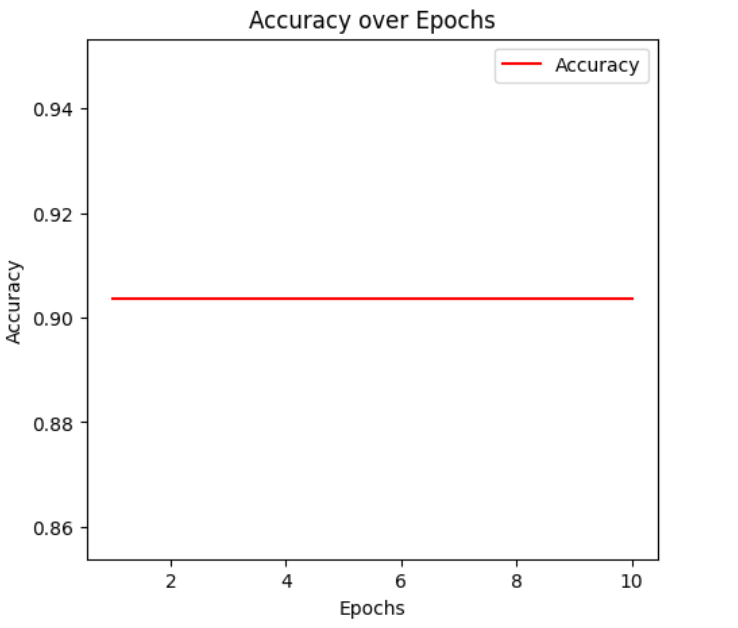
\includegraphics[width=\textwidth]{images/Results2.PNG}
        \caption{Accuracy of Model over 10 iterations}
        \label{fig:accuracy-1}
    \end{subfigure}
    
    \caption{Training Loss (a) and Accuracy (b) over 10 iterations of Federated Neural Networks Model}
    \label{fig:results-1}
\end{figure*}


\begin{figure*}[h]
    \centering
    \begin{subfigure}[b]{0.42\textwidth}
        \centering
        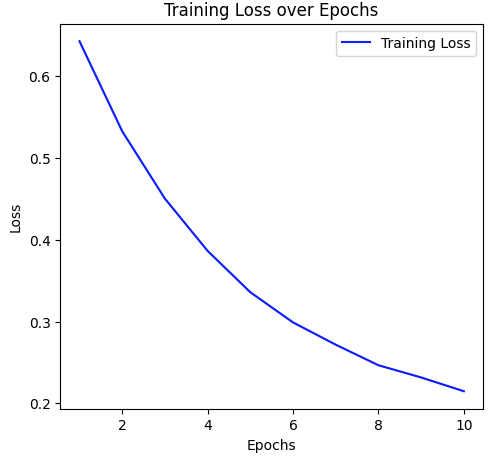
\includegraphics[width=\textwidth]{images/results3.png}
        \caption{Training Loss over 10 iterations}
        \label{fig:loss-2} % Corrected label
    \end{subfigure}
    \hfill
    \begin{subfigure}[b]{0.43\textwidth}
        \centering
        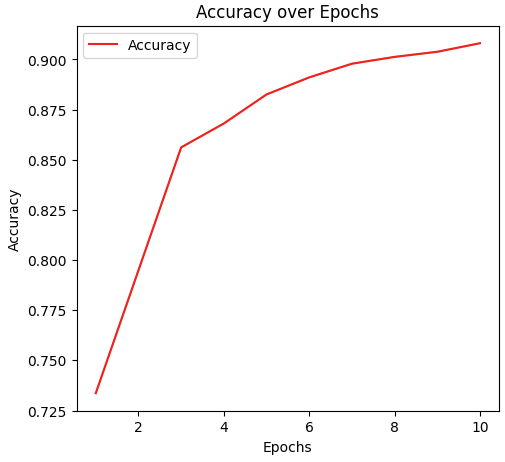
\includegraphics[width=\textwidth]{images/results4.png}
        \caption{Accuracy of Model over 10 iterations}
        \label{fig:accuracy-2}
    \end{subfigure}
    
    \caption{Training Loss (a) and Accuracy (b) over 10 iterations of Federated TinyBert Classification}
    \label{fig:results-2}
\end{figure*}

\section{Conclusion \& Discussion}
In this section, we summarize the main results of our study and discuss the limitations and challenges we encountered.

\subsection{Discussion}

The results of this study highlight the significant advancements in the field of hate speech detection through the use of both centralized and federated learning models. Our experiments demonstrate that centralized models, particularly TinyBERT, achieve high accuracy across multiple datasets. However, the federated learning approaches offers a compelling alternative by maintaining high accuracy while ensuring data privacy and security across multiple clients. This dual approach showcases the potential for balancing performance with privacy, a critical consideration in the era of data-driven decision-making.

\subsection{Revisiting Objectives}

The initial objectives of this research were to identify relevant datasets, preprocess data to address the class imbalance, re-implement state-of-the-art centralized methods, adapt these models to a federated and centralized learning framework, reproduce current federated and centralized models, and compare all models fairly. Throughout the study, we successfully identified and utilized multiple datasets for hate speech detection, implemented several centralized models, including TinyBERT, and developed federated versions of these models. The comparative analysis provided insights into the trade-offs between centralized and federated approaches, fulfilling our primary research goals.

\subsection{Implications}

The implications of this study extend to both practical applications and future research directions. The successful implementation of federated learning models for hate speech detection suggests that organizations can deploy these models to improve content moderation while safeguarding user privacy. This is particularly relevant for social media platforms and other online communities. From a research perspective, the study underscores the need for further exploration of federated learning techniques, especially in handling non-IID data and enhancing model aggregation methods. The findings also highlight the importance of balancing model performance with ethical considerations such as privacy and security in machine learning applications.

\subsection{Limitations and Challenges}
During our implementation, we encountered several limitations, which are listed below. 
\begin{itemize}
    \item \textbf{Resource Limitation:} One of the main problems we encountered was related to resource limitations. First, the data size is very large, especially when we merged the datasets. Second, using TinyBERT requires significant GPU power. Since we used the free resources of Google Colab, which has a small amount of RAM and limited GPU time access, we could not experiment with more robust results using a larger number of clients and more epochs.
    \item \textbf{SOTA Comparison:} Due to time limitations, we could not compare other state-of-the-art methods and reproduce more SOTA papers.
    \item \textbf{Other NLP Models:} There are many other encoders for classifying each tweet, which we could not implement due to a lack of resources. Additionally, TinyBERT is a small model, and using the base BERT model, which is much larger, would provide a broader perspective for our work.
    \item \textbf{Server-Client Design FL:}  Due to time limitations, we only considered a virtual machine federated setup without implementing the real server-client model transfer
\end{itemize}


\subsection{Future Work}
Working on Federated Hate-Speech Recognition is an interesting topic that has many open research problems.
\begin{itemize}
    \item \textbf{Effect of Client Size:} The effect of the number of clients is important in federated settings. Due to the mentioned limitations, testing with a larger number of clients was not feasible.
    \item \textbf{Multi-Class Classification:} Our main focus is Federated Learning for binary classification. However, there are many centralized models for multi-class classification, and feeding different class types can also be a challenging problem.
    \item \textbf{Combining Generative Models for Rare Classes:} Hate-speech datasets suffer from imbalanced labels. Using deep generative models for each client can help generate rare labels.
    \item \textbf{Federated Generative Models:} Hate-speech recognition involves tabular data, and using Generative Models in a federated manner can be an interesting research problem for further exploration.
    \item \textbf{Privacy and Security:} Further research is needed on the possibility of integrity and privacy attacks when using hate-speech datasets in a federated learning manner. Comparing existing methods regarding privacy and security is crucial.
    \item \textbf{Different Aggregation Methods:} Currently, we only consider FedProx and FedAVG as our aggregation methods. Many other well-performing aggregation methods exist and can be helpful.
    \item \textbf{Non-IID Data:} Currently, we only consider IID data in our implementation. However, working with non-IID data is another possible area for exploration.
    \item \textbf{Flower:} Flower is also one of the famous Federated Learning frameworks with many different setups. Using their implementation is also recommended for future works.

\end{itemize}



\bibliography{custom.bib}
\bibliographystyle{acl_natbib}

\newpage

\appendix
\section{Data Visualization}
\label{sec:data-visualization}
One of the experiments that we did before data augmentation was data visualization for different setups before and after up-sampling. Figure \ref{fig:data-visualization-kaggle1}, Figure \ref{fig:data-visualization-kaggle2}, and Figure \ref{fig:data-visualization-davidson} are representative of each class data visualization based on different words.

\begin{figure*}[h]
    \centering
    \begin{subfigure}[b]{0.45\textwidth} % Consistent width for both subfigures
        \centering
        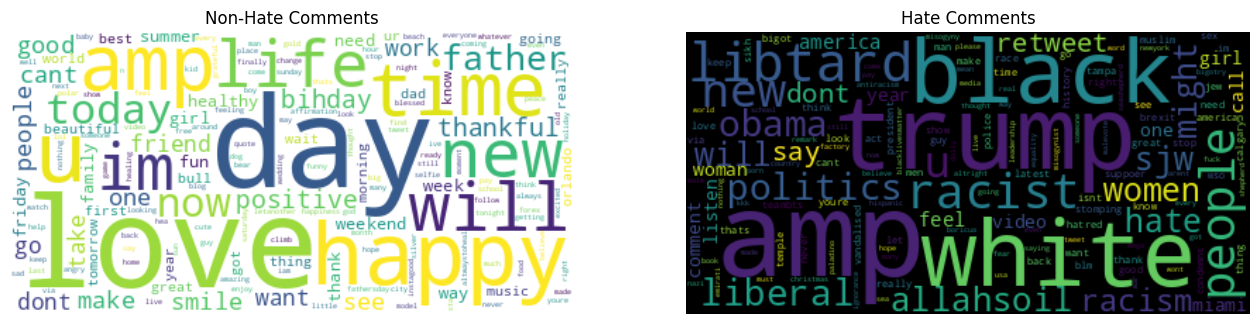
\includegraphics[width=\textwidth]{images/hatespeech_visualization/kaggle(1)-before.png}
        \caption{Before Up-Sampling}
        \label{fig:before-kaggle-1}
    \end{subfigure}
    \hfill
    \begin{subfigure}[b]{0.45\textwidth}
        \centering
        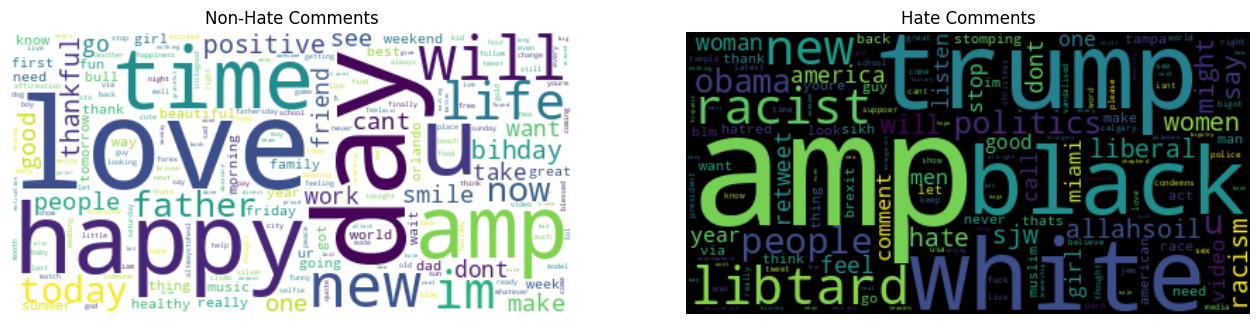
\includegraphics[width=\textwidth]{images/hatespeech_visualization/kaggle(1)-after.png}
        \caption{After Up-Sampling}
        \label{fig:after-kaggle-1}
    \end{subfigure}
    
    \caption{Kaggle(1) Dataset Each Class Visualization}
    \label{fig:data-visualization-kaggle1}
\end{figure*}

\begin{figure*}[h]
    \centering
    \begin{subfigure}[b]{0.45\textwidth}
        \centering
        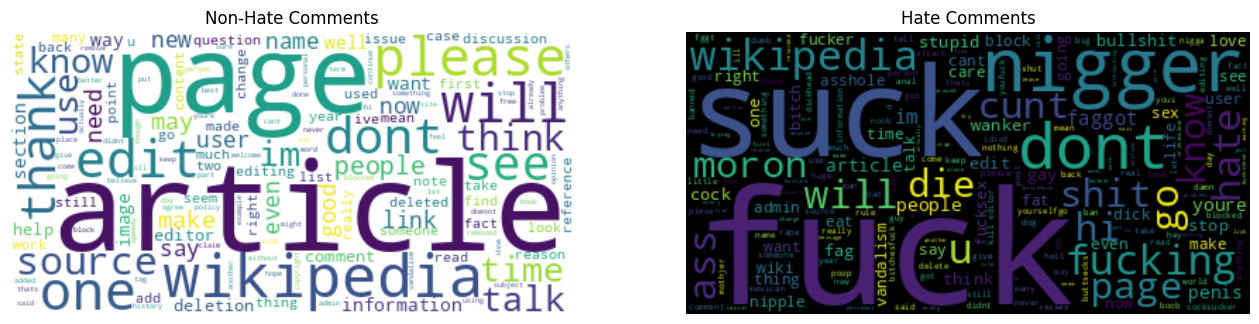
\includegraphics[width=\textwidth]{images/hatespeech_visualization/kaggle(2)-before.png}
        \caption{Before Up-Sampling}
        \label{fig:before-kaggle-2} % Corrected label
    \end{subfigure}
    \hfill
    \begin{subfigure}[b]{0.45\textwidth}
        \centering
        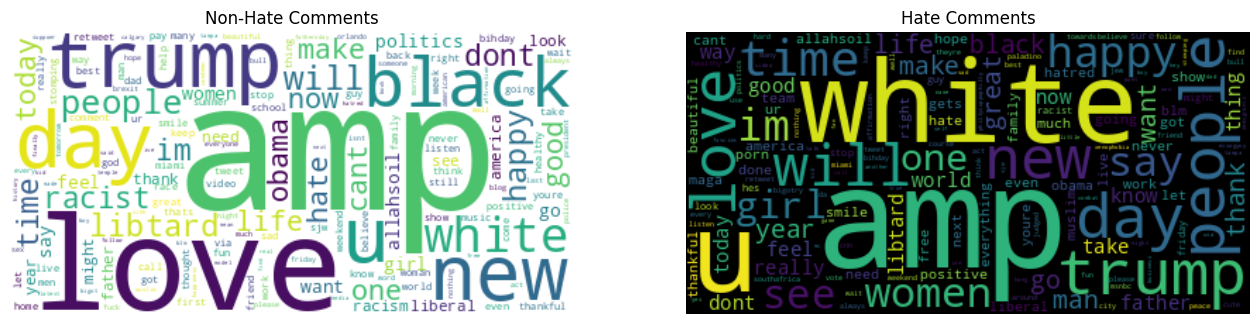
\includegraphics[width=\textwidth]{images/hatespeech_visualization/kaggle(2)-after.png}
        \caption{After Up-Sampling}
        \label{fig:after-kaggle-2}
    \end{subfigure}
    
    \caption{Kaggle(2) Dataset Each Class Visualization}
    \label{fig:data-visualization-kaggle2}
\end{figure*}

\begin{figure*}[h]
    \centering
    \begin{subfigure}[b]{0.45\textwidth}
        \centering
        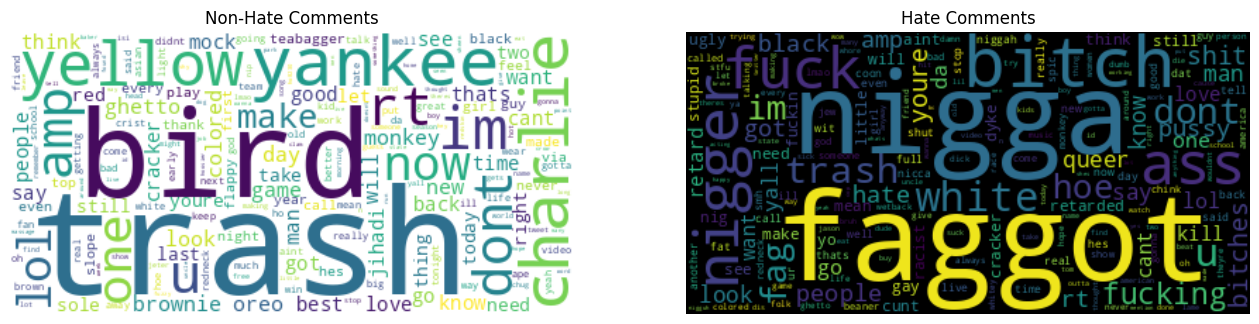
\includegraphics[width=\textwidth]{images/hatespeech_visualization/davidson(1)-before.png}
        \caption{Before Up-Sampling}
        \label{fig:before-davidson}
    \end{subfigure}
    \hfill
    \begin{subfigure}[b]{0.45\textwidth}
        \centering
        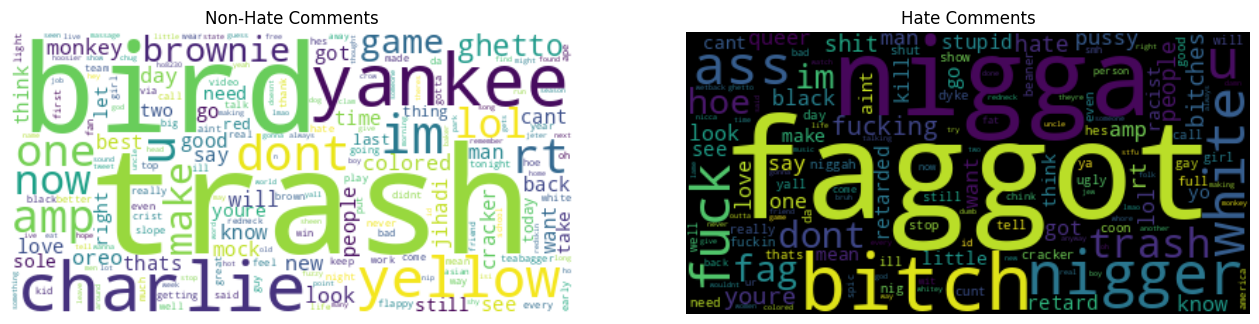
\includegraphics[width=\textwidth]{images/hatespeech_visualization/davidson(2)-after.png}
        \caption{After Up-Sampling}
        \label{fig:after-davidson}
    \end{subfigure}
    
    \caption{Davidson Dataset Each Class Visualization}
    \label{fig:data-visualization-davidson}
\end{figure*}

\section{Provided Materials}
\label{sec:materials}
We have provided our code on GitHub, which you can find at \href{https://github.com/ashkanvg/Hate-Speech-Recognizer}{https://github.com/ashkanvg/Hate-Speech-Recognizer}. Also, all of the datasets are available at \href{https://drive.google.com/drive/folders/1yrHJnPINYEEe674dYridJc23odxYG5h6?usp=sharing}{Google Drive}.


\section{Individual Efforts}
In this section, we summarize the main contribution of each person in the group. 

\subsection{Ashkan Vedadi Gargary}
My contributions to the project were primarily focused on the centralized learning aspect, emphasizing the exploration of different models and leveraging the BERT classifier. Additionally, I was responsible for federating the best-centralized model (TinyBERT) and evaluating its accuracy in a federated learning setup. Part of my role also involved reviewing related works to identify relevant datasets and models for further research.

Throughout the project, collaboration was key. We worked closely as a team, with each member making equal contributions to the project report and various parts of the implementation. We supported each other in overcoming challenges, ensuring a smooth and effective workflow.

\subsection{Aditya Mohan Gupta}

Focused on the federated learning aspect of the project, with an emphasis on hate speech detection. Conducted an extensive review of various datasets suitable for federated learning applications. Undertook a thorough analysis of existing literature to comprehend the implementation and mechanics of federated learning frameworks. Developed and implemented the code for training and evaluating the federated learning model. Collaborated closely with Ashkan, who provided valuable assistance throughout the project. Contributed significantly to the composition of the project report and the preparation of the presentation materials.

\end{document}
